\documentclass[border=4pt]{standalone}

\usepackage{tikz}

\definecolor{otblue}{HTML}{0072B2}
\definecolor{otorange}{HTML}{E69F00}
\definecolor{otteal}{HTML}{009E73}
\definecolor{otpurple}{HTML}{CC79A7}
\definecolor{otgray}{HTML}{5A5A5A}

\begin{document}
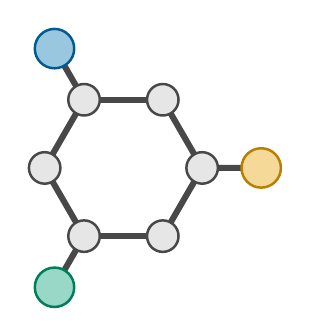
\begin{tikzpicture}[line width=0.9pt]
  \foreach \p/\q in {0/1,1/2,2/3,3/4,4/5,5/0}{\draw[otgray!80!black, line width=2.2pt] (\p*60:1) -- (\q*60:1);}
  \draw[otgray!80!black, line width=2.2pt] (0:1) -- (0:1.75) (120:1) -- (120:1.75) (240:1) -- (240:1.75);
  \foreach \a in {0,60,...,300}{\filldraw[draw=otgray!80!black, fill=otgray!15] (\a:1) circle[radius=0.2];}
  \foreach \a/\c in {0/otorange,120/otblue,240/otteal}{\filldraw[draw=\c!80!black, fill=\c!40] (\a:1.75) circle[radius=0.25];}
\end{tikzpicture}
\end{document}
